% Copyright 2004 by Till Tantau <tantau@users.sourceforge.net>.
%
% In principle, this file can be redistributed and/or modified under
% the terms of the GNU Public License, version 2.
%
% However, this file is supposed to be a template to be modified
% for your own needs. For this reason, if you use this file as a
% template and not specifically distribute it as part of a another
% package/program, I grant the extra permission to freely copy and
% modify this file as you see fit and even to delete this copyright
% notice. 

\documentclass{beamer}

% There are many different themes available for Beamer. A comprehensive
% list with examples is given here:
% http://deic.uab.es/~iblanes/beamer_gallery/index_by_theme.html
% You can uncomment the themes below if you would like to use a different
% one:

%\usetheme{AnnArbor}
%\usetheme{Antibes}
%\usetheme{Bergen}
%\usetheme{Berkeley}
%\usetheme{Berlin}
%\usetheme{Boadilla}
%\usetheme{boxes}
%\usetheme{CambridgeUS}
%\usetheme{Copenhagen}
%\usetheme{Darmstadt}
%\usetheme{default}
%\usetheme{Frankfurt}
%\usetheme{Goettingen}
%\usetheme{Hannover}
%\usetheme{Ilmenau}
%\usetheme{JuanLesPins}
%\usetheme{Luebeck}
\usetheme{Madrid}
%\usetheme{Malmoe}
%\usetheme{Marburg}
%\usetheme{Montpellier}
%\usetheme{PaloAlto}
%\usetheme{Pittsburgh}
%\usetheme{Rochester}
%\usetheme{Singapore}
%\usetheme{Szeged}
%\usetheme{Warsaw}
\colorlet{beamer@blendedblue}{green!40!black}
\usepackage[3D]{movie15}
\usepackage{cancel}
\setbeamertemplate{caption}[numbered]{}% Number float-like environments
\usepackage{pgf}
\usepackage{color}
\usepackage{listings}

\title[twoPhasePBMFoam]{The implementation of quadrature based moment methods in twoPhaseEulerFoam}

% A subtitle is optional and this may be deleted
%\subtitle{OpenFOAM solver CFD_PBM}


\author[Ehsan Askari]{Ehsan Askari}
% - Give the names in the same order as the appear in the paper.
% - Use the \inst{?} command only if the authors have different
%   affiliation.

%\institute[Sherbrooke University] % (optional, but mostly needed)
%{
  
%  Department of Chemical Engineering\\
%  Sherbrooke University
%}
% - Use the \inst command only if there are several affiliations.
% - Keep it simple, no one is interested in your street address.

\date{28th Oct, 2016}
% - Either use conference name or its abbreviation.
% - Not really informative to the audience, more for people (including
%   yourself) who are reading the slides online

%\subject{Theoretical Computer Science}
% This is only inserted into the PDF information catalog. Can be left
% out. 

% If you have a file called "university-logo-filename.xxx", where xxx
% is a graphic format that can be processed by latex or pdflatex,
% resp., then you can add a logo as follows:

\pgfdeclareimage[height=0.8cm]{university-logo}{university-logo-filename}
%\logo{\pgfuseimage{university-logo}}{\pgfbox[right,base]}

%\logo{\pgfputat{\pgfxy(0,8)}{\pgfbox[right,base]{
\includegraphics[height=0.63cm]{/home/ehsan/Desktop/logo2.png}}}}


%\logo{
\includegraphics[height=0.8cm]{university-logo-filename}\vspace{220pt}}

% Delete this, if you do not want the table of contents to pop up at
% the beginning of each subsection:
\AtBeginSubsection[]
{
  \begin{frame}<beamer>{Outline}
    \tableofcontents[currentsection,currentsubsection]
  \end{frame}
}

% Let's get started
\begin{document}

\begin{frame}
  \titlepage
\end{frame}

\begin{frame}{Outline}
  \tableofcontents
  % You might wish to add the option [pausesections]
\end{frame}

% Section and subsections will appear in the presentation overview
% and table of contents.
\section{Introduction}

\begin{frame}{The updated plan of project}

  \begin{figure}
  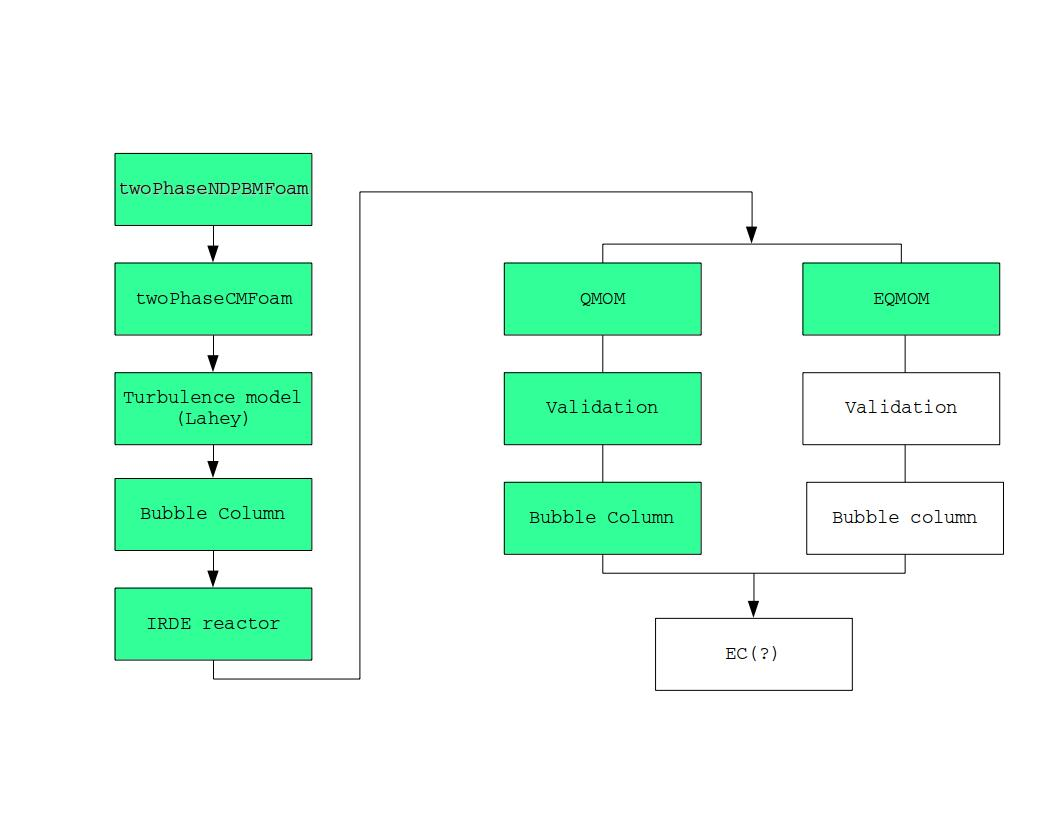
\includegraphics[width=0.9\linewidth]{plan.jpg}
  \end{figure} 

\end{frame}

\begin{frame}{Population balance methods}

\begin{itemize}
\item Number density approach
\item Interfacial Area Transport Equation (IATE)
\item Class Method (CM)
\item Quadrature Method of Moments (QMOM) 


\end{itemize}


\begin{equation*}
n(L;\textbf{x},t)=\sum_{i=1}^{N}W(i)\times \delta(L-L_i)
\end{equation*}

\begin{equation*}
m_k=\int_{0}^{+\infty}n(L;\textbf{x},t)L^kdL
\end{equation*}


\end{frame}

\section{Quadrature method of moments (QMOM)}


%%%%%%%%%%%%%%%%%%%%%%%%%%%%%%%%%%%%%%%%%%%%%%%%%%%%%%%%%%%%%%%%%%
\begin{frame}{Quadrature method of moments, McGraw (1997)}

\begin{equation*}
m_k=\int_{0}^{+\infty}n(L;\textbf{x},t)L^kdL
\end{equation*}

\begin{equation*}
m_k =\sum_{i=1}^{N}L_i^k w_i(t,x), \ \ \ \ \ \ k=0, 1, 2, ..., 2N-1
\end{equation*}

\begin{equation*}
\frac{\partial m_k (t,x)}{\partial t}+\nabla .(\textbf{U}^{(k)}m_k(t,x)) = \overline{S}_k 
\end{equation*}


\begin{figure}
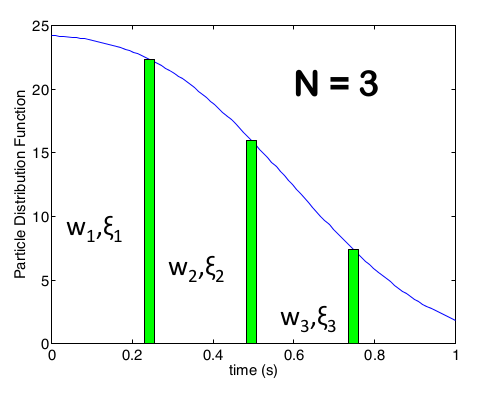
\includegraphics[width=0.3\linewidth]{nodes.png}
\end{figure}
  
\end{frame}

\begin{frame}{Source terms in QMOM}

\begin{equation*}
\overline{S}_k =\overline{B}_{ag,k}-\overline{D}_{ag,k} +\overline{B}_{br,k}-\overline{D}_{br,k} 
\end{equation*}

\begin{equation*}
\overline{B}_{ag,k} =\frac{1}{2}\sum_{i}^{N}\sum_{j}^{N} W_i W_j {(L_i^3+L_j^3)}^{k/3} \textcolor{green}{a_{ij}}
\end{equation*}

\begin{equation*}
\overline{D}_{ag,k} =\sum_{i}^{N}\sum_{j}^{N} W_i W_j L_i^k \textcolor{green}{a_{ij}}
\end{equation*}

\begin{equation*}
\overline{B}_{br,k} =\sum_{i}^{N} W_i \textcolor{blue}{\overline{b}^{(k)}_i} \textcolor{red}{\beta_i}
\end{equation*}

\begin{equation*}
\overline{D}_{br,k} =\sum_{i}^{N} L_i^k  W_i \textcolor{red}{\beta_i} 
\end{equation*}

\end{frame}

\begin{frame}{QMOM Validation (D. L. Marchisio et al. (2003))}

\begin{equation*}
\frac{\partial m_k (t,x)}{\partial t} = \overline{B}_{ag,k}-\overline{D}_{ag,k} +\overline{B}_{br,k}-\overline{D}_{br,k}
\end{equation*}

\begin{itemize}
\item Aggregation kernel: 
\end{itemize}
\begin{center}
$\textcolor{green}{a_{ij}}=a(L_i,L_j)=0.02$
\end{center}

\begin{itemize}
\item Breakage kernel: 
\end{itemize}
\begin{center}
$\textcolor{red}{\beta_{i}}=\beta(L_i)=1$
\end{center}

\begin{itemize}
\item Daughter distribution: 
\end{itemize}
\begin{center}
$\textcolor{blue}{\overline{b}^{(k)}_i}=2^{(3-k)/3}L_i^k$
\end{center}

\begin{itemize}
\item Moment initialization: 
\end{itemize}
\begin{center}
$m_k=0, k=0,1,...,5$
\end{center}

\end{frame}


\begin{frame}{Comparison}
   \begin{figure}[H]
  
    \includegraphics[width=0.47\textwidth,keepaspectratio]{m0}
    \includegraphics[width=0.47\textwidth,keepaspectratio]{d34}
\end{figure} 
\end{frame}

\begin{frame}{Coupling QMOM and twoPhaseEulerPBMFoam (1)}
\begin{columns}

\begin{column}{0.3\textwidth}

  \begin{figure}
  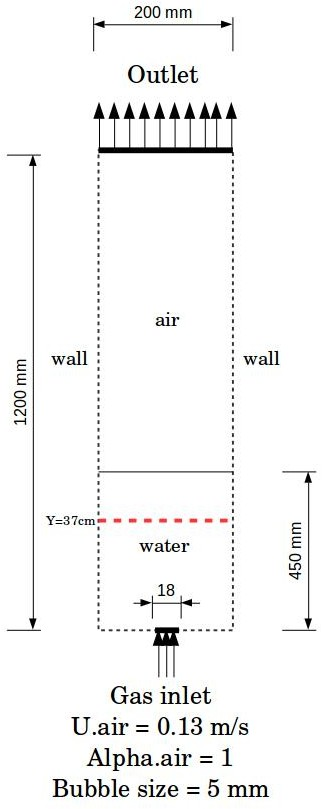
\includegraphics[width=0.8\linewidth]{y37.jpg}
  \end{figure} 

\end{column}  

\begin{column}{0.9\textwidth}

\begin{itemize}

\item Liquid (water) : continuous phase

\item Gas (air) : dispersed phase

\item $\textcolor{red}{d} \Rightarrow QMOM$ $\boxed{d =  \frac{m3}{m2}}$ 

\item Liquid: Turbulent 

\item Gas: Laminar 

\item Incompressible fluids

\item PDE for moments:


          fvm::ddt(m[i])+ fvm::div(phia, m[i], fScheme)- fvm::Sp(fvc::div(phia), m[i])

     

\end{itemize}

\end{column}

\end{columns}

\end{frame}


\begin{frame}{Coupling QMOM and twoPhaseEulerPBMFoam (2)}
\begin{equation*}
\frac{\partial m_k (t,x)}{\partial t}+\nabla .(\textbf{U}^{(k)}m_k(t,x)) = \overline{B}_{ag,k}-\overline{D}_{ag,k} +\overline{B}_{br,k}-\overline{D}_{br,k}
\end{equation*}

\begin{itemize}
\item Aggregation kernel: 
\end{itemize}
\begin{center}
$\textcolor{green}{a_{ij}}=a(L_i,L_j)=0.02$ 
\end{center}

\begin{itemize}
\item Breakage kernel:
\end{itemize}
\begin{center}
$\textcolor{red}{\beta_{i}}=\beta(L_i)=1$ 
\end{center}

\begin{itemize}
\item Daughter distribution: 
\end{itemize}
\begin{center}
$\textcolor{blue}{\overline{b}^{(k)}_i}=2^{(3-k)/3}L_i^k$
\end{center} 

\begin{center}
\boxed{Divergence}
\end{center}

\end{frame}

\begin{frame}{Coupling QMOM and twoPhaseEulerPBMFoam (3)}
\begin{equation*}
\frac{\partial m_k (t,x)}{\partial t}+\nabla .(\textbf{U}^{(k)}m_k(t,x)) = \overline{B}_{ag,k}-\overline{D}_{ag,k} +\overline{B}_{br,k}-\overline{D}_{br,k}
\end{equation*}

\begin{itemize}
\item Aggregation kernel: 
\end{itemize}
\begin{center}
$\textcolor{green}{a_{ij}}=a(L_i,L_j)\Rightarrow$ Luo aggregation kernel
\end{center}

\begin{itemize}
\item Breakage kernel: Luo breakage kernel
\end{itemize}
\begin{center}
$\textcolor{red}{\beta_{i}}=\beta(L_i)\Rightarrow$ Luo breakage kernel
\end{center}

\begin{itemize}
\item Daughter distribution: 
\end{itemize}
\begin{center}
$\textcolor{blue}{\overline{b}^{(k)}_i}=2^{(3-k)/3}L_i^k$
\end{center} 
\end{frame}

\begin{frame}{Validation QMOM+twoPhaseEulerFOAM}
   \begin{figure}[H]
     \includegraphics[width=0.8\textwidth,keepaspectratio]{comparison}

\end{figure} 

\end{frame}
%%%%%%%%%%%%%%%%%%%%%%%%%%%%%%%%%%%%%%%%%%%%%%%%%%%%%%%%%%%%%%%%%%%%



\begin{frame}{Result QMOM+twoPhaseEulerFOAM}

   \begin{figure}[H]
     \includegraphics[width=0.58\textwidth,keepaspectratio]{m0contour.eps} 
     \includegraphics[width=0.58\textwidth,keepaspectratio]{alpha.eps}

\end{figure} 

\end{frame}

\section{Extended Quadrature method of moments (EQMOM)}

\begin{frame}{Extended Quadrature Method of Moments (EQMOM), C. Yuan et al. (2012) }

\begin{itemize}
\item Quadrature method of moments (QMOM) 
\end{itemize}

\begin{equation*}
n(L;\textbf{x},t)=\sum_{i=1}^{N}W(i)\times \textcolor{blue}{\delta_{\sigma}(L-L_i)}
\end{equation*}


\begin{itemize}
\item Extended Quadrature Method of Moments (EQMOM) 
\end{itemize}

\pause

\begin{equation*}
\lim_{\delta \to 0} \delta_{\sigma}(L,L_i) = \delta(L-L_i)
\end{equation*}

\begin{equation*}
n(L;\textbf{x},t)=\sum_{i=1}^{N}W(i)\times \textcolor{red}{\delta_{\sigma}(L,L_i)}
\end{equation*}

\end{frame}

\begin{frame}{Source terms in EQMOM}

\begin{equation*}
\overline{S}_k =\overline{B}_{ag,k}-\overline{D}_{ag,k} +\overline{B}_{br,k}-\overline{D}_{br,k} 
\end{equation*}

\begin{equation*}
\overline{B}_{ag,k} =\frac{1}{2}\sum_{\alpha_1=1}^{N}\sum_{\beta_1=1}^{N_{\alpha}} W_{\alpha_1} W_{\alpha_1 \beta_1} \sum_{\alpha_2=1}^{N}\sum_{\beta_2=1}^{N_{\alpha}} W_{\alpha_2} W_{\alpha_2 \beta_2}  {(L_{\alpha_1\beta_1}^3+L_{\alpha_2\beta_2}^3)}^{k/3} \textcolor{green}{a_{\alpha_1\beta_1\alpha_2\beta_2}}
\end{equation*}

\begin{equation*}
\overline{D}_{ag,k} =\sum_{\alpha_1=1}^{N}\sum_{\beta_1=1}^{N_{\alpha}} L^k_{\alpha_1\beta_1} W_{\alpha_1} W_{\alpha_1 \beta_1} \sum_{\alpha_2=1}^{N}\sum_{\beta_2=1}^{N_{\alpha}} W_{\alpha_2} W_{\alpha_2 \beta_2} \textcolor{green}{a_{\alpha_1\beta_1\alpha_2\beta_2}}
\end{equation*}

\begin{equation*}
\overline{B}_{br,k} =\sum_{\alpha_1=1}^{N}\sum_{\beta_1=1}^{N_{\alpha}} W_{\alpha} W_{\alpha \beta} \textcolor{blue}{\overline{b}^{(k)}_{\alpha \beta}} \textcolor{red}{\beta_{\alpha \beta}}
\end{equation*}

\begin{equation*}
\overline{B}_{br,k} =\sum_{\alpha_1=1}^{N}\sum_{\beta_1=1}^{N_{\alpha}} W_{\alpha} W_{\alpha \beta} L^k_{\alpha\beta} \textcolor{red}{\beta_{\alpha \beta}} 
\end{equation*}

\end{frame}

\begin{frame}{EQMOM algorithm}

\begin{enumerate}
\item Guess $\sigma$, compute the $2n$ moments $m_k^{*}$ for $k=0,...,2n-1$
\item Use PD or Wheeler algorithm with $m_k^{*}$ for for $k=0,...,2n-1$ to find $n$ weights and $n$ abscissas $L_{\alpha}$
\item Compute $m_{2n}^*$ using $w_{\alpha}$ and $L_{\alpha}$
\item Construct $J_n(\sigma)$ from $m^{*}$ and $\sigma$
\item Find root to achieve 
\end{enumerate}

 
\end{frame}

\begin{frame}{EQMOM and Normal distribution}

\begin{equation*}
m_0^*=m_0
\end{equation*}

\begin{equation*}
m_1^*=m_1
\end{equation*}

\begin{equation*}
m_2^*=m_2-m_0^*\sigma^2
\end{equation*}

\begin{equation*}
m_3^*=m_3-3m_1^*\sigma^2
\end{equation*} 

\begin{equation*}
m_4^*=m_4-6m_2^*\sigma^2-3m_0^*\sigma^2
\end{equation*} 

\begin{equation*}
m_5^*=m_5-10m_3^*\sigma^2-15m_1^*\sigma^4
\end{equation*} 

\begin{equation*}
m_6^*=m_6-15m_4^*\sigma^2-45m_2^*\sigma^4-15m_0^*\sigma^6
\end{equation*} 


\end{frame}

\begin{frame}{EQMOM and Normal distribution $N=1$, $\sigma=1$, $\mu=5$}

\begin{center}
$m_0=1.0$, $m_1=5.0$, $m_2=33.33$
\end{center}

\begin{center}
$\Downarrow$
\end{center}

\begin{center}
$L_1=5$ and $w_1=1$
\end{center}

\begin{equation*}
m_2^*=\sum_{\alpha=1}^{N}W_{\alpha} L_\alpha^2=w_1 \times L_1^2
\end{equation*} 

\begin{equation*}
m_2^*=m_2-m_0^*\sigma^2
\end{equation*}

\begin{equation*}
J_n(\sigma)=w_1 \times L_1^2-m_2-m_0^*\sigma^2
\end{equation*}

\begin{center}
$\boxed{\sigma^2=8.33}$
\end{center}

\end{frame}



%%%%%%%%%%%%%%%%%%%%%%%%%%%%%%%%%%%%%%%%%%%%%%%%%%%%%%%%%%%%%%%%%%%%


\begin{frame}{EQMOM+twoPhaseEulerFoam}

   \begin{figure}[H]
     \includegraphics[width=0.8\textwidth,keepaspectratio]{sigma.eps} 
     
\end{figure}
   
\end{frame}



\section{Conclusion}

\begin{frame}{The conclusion}

\begin{itemize}
\item Done:


\begin{itemize}
\item twoPhaseEulerPBMFoam was updated with QMOM and EQMOM
\item QMOM validation
\item twoPhaseEulerFoam+QMOM Validation
\item Initial EQMOM library
\end{itemize}
\end{itemize}

\begin{itemize}
\item Coming:


\begin{itemize}
\item Apply EQMOM source terms
\item EQMOM validation with \textbf{"Ehsan Madadi and Alberto Passalacqua (2015)"}
\end{itemize} 
\end{itemize}
\end{frame}



\begin{frame}

\begin{center}
\textbf{Thank you for your attention!}
\end{center}


\end{frame}

\begin{frame}{Appendix}

\begin{itemize}
\item Luo Breakage kernels
\end{itemize}

\begin{equation*}
\Omega_{br}(V,V')= k \int_{\zeta}^{1}\frac{{(1+\zeta)}^2}{\zeta^n} exp(-b\zeta^m)d\zeta
\end{equation*}

\begin{itemize}
\item Luo aggregation kernels
\end{itemize}

\begin{equation*}
\Omega_{ag}(V_i,V_j)= \omega_{ag} \times P_{ag} (V_i,V_j)
\end{equation*}

\end{frame}





%%%%%%%%%%%%%%%%%%%%%%%%%%%%%%%%%%%%%%%%%%%%%%%%%%%%%%%%%%%%%%%%%%%%%%%%%%%%%%%%%%%%%%%%%%%%%%%%%%%%%%%%




\end{document}
